\section{Interpretation Methods}
\label{sec:interpretation_methods}

% All explanation methods are post hoc
There exists a variety of definitions in the vastly expanding research field of XAI, and the concept of \textit{interpretability} still has no formal commonly used technical meaning \cite{lipton2018mythos}. To build on the common ground of existing research, this paper follows the terminoloqy of \cite{arrieta2020explainable}.
The authors make a distinction between the related but different concepts of \textit{interpretability} and \textit{explainibility}.

\mypar{Interpretability} refers to the the extent to which cause and effect can be observed in a model, which can be translated to uncovering \textit{why} a model made prediction $y$ to an input $\mathbf{x}$. Consider the example of image classification from \autoref{fig:bb}. Here, interpretability would mean that if a cat is present in the image (the cause), the model classifies it to the category 'cat' (the effect). Now imagine we find that the model takes the green meadow in the image as evidence to predict 'cat', and not the cat itself, there is a lack of interpretability, as other features are learned as important than the features that are truly important. This toy example is in fact a common problem in image classification: the over-reliance of models on image background, rather than on objects in the foreground, has been observed for the task of image classification \cite{xiao2020noise}.% Note that interpretabe AI cannot verify if the learned relationships between features and outputs is truly causal (tha meadow in tha image can be correlated to the image category, e.g. when most images depictiong a cat shows cats on green meadows. This is a correlation of features but not necessarily a causilaty in tha sense of 'meadow --> cat'. ) https://www.pnas.org/content/pnas/116/44/22071.full.pdf causal inference

\mypar{Explainibility} on the other hand spans methods to uncover \textit{how} a model makes predictions, meaning to observe the inner workings of a model and to literally explain what is happening.

% The notion of these two concepts can be nicely explained by the comparison between deep neural networks and (shallow) decision trees. 
% Within a decision tree, there exists a distinct set of rules. The date will be split at each node into subsets and the leaf node hold the predicted outcome. All edges are connected by a logical 'AND'. Thus, cause and effect in a shallow decision tree are easy to observe and visualize, and thus the model is interpretable. 
% However, a deep neural network, holding millions to billions of parameters in several layers, there are many neurons impacting the prediction to in order to directly attribute the impact of individual input features.  

While both concepts seem to be important for the general objective of explainable artificial intelligence, this paper focuses on interpretability. 
High interpretability is desired as it can help to to uncover biases in the model. Suppose a machine learning model is to be deployed for the task of income prediction based on features such as age, race, gender, education and hours of work per week. The performance of the system would mainly be evaluated in terms oft the predictive accuracy and the fairness of the system. The former can be evaluated with metrics, such as accuracy on a held-out test set. For the latter, interpretability methods might be applied to observe which input features are used by the model to predict the income. 
% TODO note here that tha data from adult_income do actually not allow for these features to be more important than others. 
If the model uses sensitive features, such as sex and race as important features, it is systematically biased and thus unfair. 


%%%%% TAXONOMY
This section offers a taxonomy for machine learning interpretation methods.

There are essentially two ways to achieve interpretability: (1) to use inherently interpretable models or (2) to post-process a model in a fashion that allows to yield insights. The former is known as the development of \textit{surrogate} models and more generally described as \textit{model-agnostic} methods. Option (2) is known as \textit{model-transparent} methods. 

A further categorization can be made based on the scope of interpretations: \textit{Local} methods aim at interpretations that are true for a single data points and its neighbors. 
\textit{Global} methods aim at gaining interpretations that are valid for most data points in a class \cite{kim2018interpretability, nguyen2017plug, yosinski2015understanding}. The interpretation methods discussed within this paper mostly fall into the class of local explanation methods \cite{ribeiro2016should, lundberg2017unified}. % TODO cite lrp, ...

Explanation methods aim at making complex and inherently uninterpretable black box models interpretable by creating human readable visualizations. 
A frequently used type of explanation methods are feature attributions mapping each input feature to a numeric score. This score should quantify the importance of the feature relative to the model output. The resulting attribution map is then visualized as a heatmap projected onto the input sample to interpret the input attributes regarding which ones are the most helpful for forming the final prediction. 

\textbf{Definition 1: Interpretation Method}\\
We consider a neural network $N: \mathbb{R}^d \to \mathbb{R}^k$. For the task of image classification, $N$ classifies an input image $\mathbf{x}\in \mathbb{R}$ in $k$ categories where the prediction $f_N(\mathbf{x})=y \in \{1, ..., K\}$ is given by $y = arg max_i f_N(\mathbf{x})_i$.

Given the neural network $N$, it's input vector $\mathbf{x} \in \mathbb{R}^d$ and the the neural networks prediction for input $\mathbf{x}$, $f_N(\mathbf{x})=y$, an interpretation method $\mathcal{I}$ determines why label $y$ has been chosen by $N$ for input $\mathbf{x}$. 
The interpretation is given by an output vector $\mathbf{x} \in \mathbb{R}^d$ where each entry $h_i$ is mostly a numeric value describing the relevance of an input dimension $x_i$ of $\mathbf{x}$ for $f_N(\mathbf{x})$. 
As $\mathbf{x}$ has the same dimensions as the input $\mathbf{x}$ it can be mapped to the input, overlaying $\mathbf{x}$ as a heatmap, where the color value represents the importance of feature $x_i$ towards the prediction $f_N(\mathbf{x})$.

An example is given in TODO. Higher values, implying a stronger relative importance for making the prediction $f_N(\mathbf{x})$, is depicted in TODD color. 

%%%%%%%%%%
% \subsection{Model Assumptions}
% \label{subsec:model_assumptions}


While all explanation methods try to obtain importance measures for the network prediction, they differ with respect to how these measures are obtained. 
\cite{evaluating_explanations_security} propose two major categories for explanation strategies, namely \textit{black-box} explanation methods and \textit{white-box} explanation methods. 
While black-box interpretations assume no knowledge about the underlying model, white-box methods only work by using the model parameters. 

This terminology of discriminating between bb and wb models may not be confused with the nature of the underlying models: Models still remain of black-box nature even though a white-box method may contribute to making the decision making process of such a model more insightful. % The opposite ofblack-box-nessistransparency,i.e., the search for a direct understanding of the mechanism by which a model works [5] 


The following section details the two categories and will give examples of the state-of-the-art interpretation methods within each group. 

% \noindent\textbf{Black-box Methods.} Black-box interpretations assume no knowledge about the model thus treating it as a black-box. The underlying model is approximated by learning it's behavior with an interpretable model, e.g. a linear model. As the model itself does not need to be known for using such a model-agnostic approach, thy can be used in scenarios where the model itself is not directly accessible. A black-box interpretation offers the big advantage to be applicable to any model.


% \noindent\textbf{White-box Methods.} On the other side are white-box interpretations, where the model is known with all its parameters. Thus, the explanations can be directly computed by using the model instead of relying on an approximation of $f_N$ as within the black-box models. As within these white-box models, tha model parameters can be used for calculating the interpretations, these methods are also named gradient or saliency map based methods. 


\subsection{Model-agnostic methods.}
\label{subsec:bb_methods}

% https://proceedings.neurips.cc//paper/2020/file/2c29d89cc56cdb191c60db2f0bae796b-Paper.pdf p. 4 
Model-agnostic interpretations assume no knowledge about the model thus treating it as a black box. The underlying model is approximated by learning it's behavior with an interpretable model, e.g. a linear model. The interpretable model is also dubbed the 'surogate' model. The common approach for learning the surrogate is to approximate the relationship between the input samples and the corresponding prediction by tho model.
As the model itself does not need to be known, these approaches can be used in scenarios where the model itself is not directly accessible. Model-agnostic interpretations are fairly popular and are used in a wide range of applications, ranging from finance and law to medicine and chemistry \cite{elshawi2019interpretability, whitmore2016mapping}. 

A black-box interpretation offers the great advantage of being applicable to any model and offers simplicity because the interpretation is embedded in the model. However, this option of gaining interpretability might be costly for users that already have a high performing model. For this reason, growing need for methods exists that can be applied without retraining or modifying the underlying model.

% https://arxiv.org/pdf/1911.02508.pdf
% Due to their generality, thesemethods have been used to explain a number of classifiers, suchas neural networks and complex ensemble models, and in variousdomains ranging from law, medicine, finance, and science [7,10,25]


\mypar{LIME.}
Local Interpretable Model-agnostic Explanations (LIME) \cite{ribeiro2016should} perturbs the input and observes how the predictions change. In image classification,  LIME creates a set of perturbed instances by dividing the input image into interpretable components (contiguous superpixels), and runs each perturbed instance through the model26
to get a probability.

\autoref{fig:lime_cat} shows an example of LIME applied to an image and the neural network model Inception-v3 \cite{szegedy2016rethinking}. 


\begin{figure}[ht]
  \centering
  \begin{subfigure}{0.32\linewidth}
    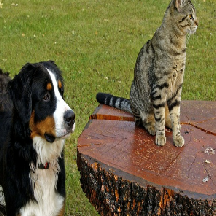
\includegraphics[width=\linewidth]{figures/lime_orig.png}
    \caption{Original}
    \label{fig:bird-a}
  \end{subfigure}
  \begin{subfigure}{0.32\linewidth}
    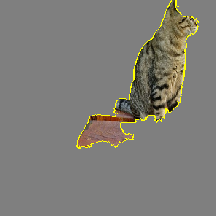
\includegraphics[width=\linewidth]{figures/lime_cat_mask.png}
    \caption{Mask}
    \label{fig:bird-a}
  \end{subfigure}
  \begin{subfigure}{0.32\linewidth}
    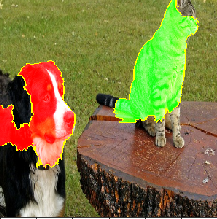
\includegraphics[width=\linewidth]{figures/lime_cat_map.png}
    \caption{Saliency Map}
    \label{fig:bird-a}
  \end{subfigure}
  \caption{Visualization of LIME.}\label{fig:lime_cat}
  \vspace{-0.3cm}
\end{figure}

% https://github.com/marcotcr/lime
% While the model may be very complex globally, it is easier to approximate it around the vicinity of a particular instance. While treating the model as a black box, we perturb the instance we want to explain and learn a sparse linear model around it, as an explanation. The figure below illustrates the intuition for this procedure. The model's decision function is represented by the blue/pink background, and is clearly nonlinear. The bright red cross is the instance being explained (let's call it X). We sample instances around X, and weight them according to their proximity to X (weight here is indicated by size). We then learn a linear model (dashed line) that approximates the model well in the vicinity of X, but not necessarily globally.


\mypar{SHAP.} SHAP \cite{lundberg2017unified}, short for SHapley Additive exPlanations, calculates an additive feature importance score for each prediction with a set of desirable properties, such as local accuracy or consistency that its antecendants lacked. 


\subsection{Model-transparent methods. }
\label{subsec:wb_methods}

On the other side are model-transparent, or white box, methods where the underlying model is known with all its parameters. Thus, the interpretation can be directly computed by using the model instead of relying on an approximation of $f_N$ as within the black-box methods. These methods typically rely on the relationship between an input sample, the underlying model's prediction and the associated activations of the models hidden layers. Most methods in this area aim to highlight the features of the input that are important the prediction.  
An example for model-transparent methods are gradient based and saliency map based methods. 

\mypar{Notations.}
A model-transparent interpretation method, in the following named interpreter $\mathcal{I}$, generates a heatmap
 $$h_c^\mathcal{I}(\boldsymbol{\omega}) = \mathcal{I}(\mathbf{x}, c; \boldsymbol{\omega})$$
  for a neural network with parameters $\boldsymbol{\omega}$ and class $c$. The heatmap is a vector $h_c^\mathcal{I}(\boldsymbol{\omega}) \in \mathbb{R}^d$, where the $j$-th value $h_{c, j}^\mathcal{I}(\boldsymbol{\omega})$ represents the importance score of the $j-th$ input feature $x_j$ for the final score of class $c$.

\mypar{Layer-wise Relevance Propagation (LRP)}
relies on a Taylor series close to the prediction point rather than partial derivatives atthe prediction point itself

\mypar{ Gradient-weighted Class Activation Mapping (Grad-CAM)} \cite{selvaraju2017grad}
To further improve the quality of the visualization, attribution methods suchas heatmaps, saliency maps or class activation methods (GradCAM[292]) are used. Grad-CAM uses the gradients of any target concept, flowing into the final convolutional layer to produce acoarse localization map, highlighting the important regions in the image for predicting the concept

\mypar{SimpleGrad (SimpleG)}

\mypar{Smooth Grad}